\chapter{Diamond-Square Algorithmus}
Die Vorteile des Diamond-Square Algorithmus liegen insbesondere in seinen, trotz seiner einfachen Implementierung, optisch plausiblen Ergebnissen. 
Der Algorithmus unterteilt sich pro Rekursionschritt in 2 Phasen\footnote{Auch \emph{Steps} genannt}: der Diamond und der Square Step. Das zu berechnende Höhenfeld muss dabei in der Auflösung eine Breite bzw. Höhe von $2n+1$ wobei $ n\in\mathbb{N}$ aufweisen.

Zur Initialisierung werden den vier Eckpunkte des zu berechnenden Höhenfeldes jeweils zufällige Höhenwerte zugewiesen. Außerdem wird eine von der Rekursionstiefe abhängige Offset-Funktion $O(k)=(rnd()*2-1)/2^k$ definiert, wobei rnd() einen Zufallswert zwischen 0-1(inklusive) zurückgibt.

Im Diamond Step wird nun der Mittelpunkt des Höhenfeld gesucht und mittels einer beliebigen Interpolation\footnote{In der Beispielimplementierung wurde eine billineare Interpolation gewählt} zwischen den 4 Höhenwerten der Eckpunkte ein Wert gefunden, welcher dann mit der Offset-Funktion zufällig verschoben wird.
\begin{figure}
	\centering
	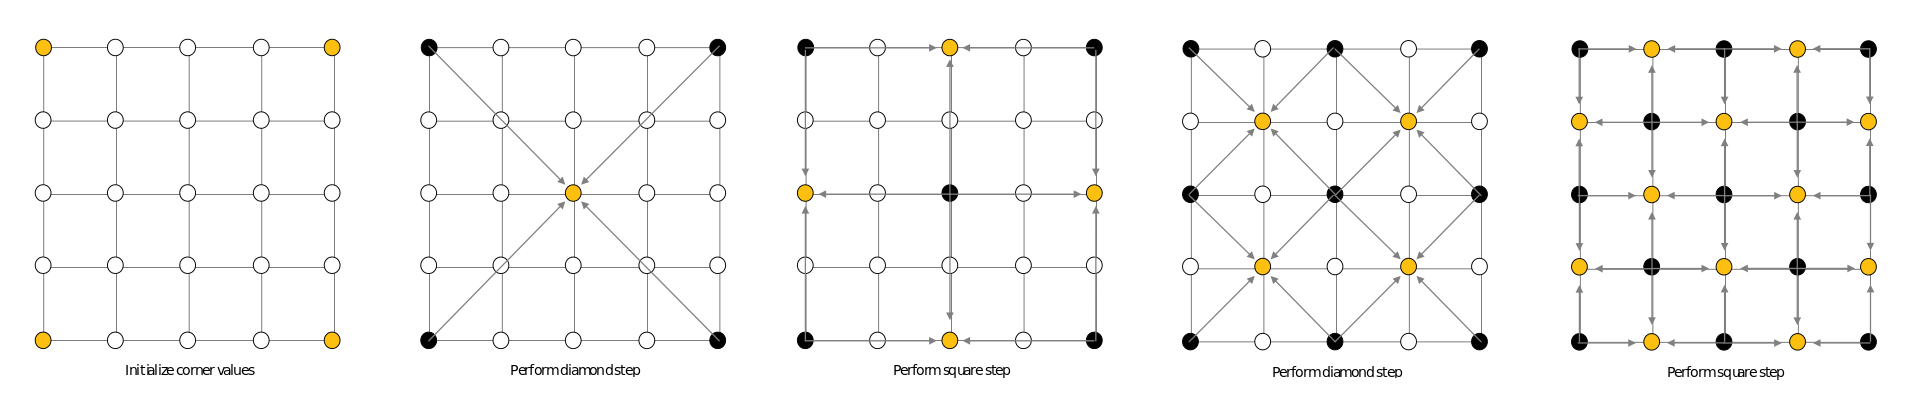
\includegraphics[width=\textwidth]{images/Diamond_Square.png}
	\caption{2 Rekursionschritte des Diamond Square Algorithmus bei einem quadratischen Höhenfeld mit der Auflösung 5x5}\label{img.dmsquare}
\end{figure}
Bei dem Square Step werden nun die jeweiligen mittleren Randpunkte zwischen den bereits initialisierten Eckpunkten durch eine einfache Interpolation zwischen den 2 nächstliegendsten Eckpunkten berechnet.
Wie in \autoref{img.dmsquare} zu sehen ergeben sich daraus 4 weitere Vierecke mit berechneten Eckpunkten, auf die der Algorithmus wieder angewandt werden kann.

Das resultierende Höhenfeld lässt sich einfach durch eine Veränderung der Offset-Funktion relativ flexibel anpassen. So besteht zum Beispiel die Möglichkeit, die Offset-Funktion von dem interpolierten Höhenwert des aktuellen Punktes abhängig so machen und so ein heterogenes Landschaftsbild zu erzeugen.

%TODO Code wie für Noise